\documentclass[]{article}
\usepackage{lmodern}
\usepackage{amssymb,amsmath}
\usepackage{ifxetex,ifluatex}
\usepackage{fixltx2e} % provides \textsubscript
\ifnum 0\ifxetex 1\fi\ifluatex 1\fi=0 % if pdftex
  \usepackage[T1]{fontenc}
  \usepackage[utf8]{inputenc}
\else % if luatex or xelatex
  \ifxetex
    \usepackage{mathspec}
  \else
    \usepackage{fontspec}
  \fi
  \defaultfontfeatures{Ligatures=TeX,Scale=MatchLowercase}
\fi
% use upquote if available, for straight quotes in verbatim environments
\IfFileExists{upquote.sty}{\usepackage{upquote}}{}
% use microtype if available
\IfFileExists{microtype.sty}{%
\usepackage{microtype}
\UseMicrotypeSet[protrusion]{basicmath} % disable protrusion for tt fonts
}{}
\usepackage[margin=1in]{geometry}
\usepackage{hyperref}
\hypersetup{unicode=true,
            pdftitle={Severe Weather Event Data Analysis - NOAA},
            pdfauthor={Sanjay Somraj},
            pdfborder={0 0 0},
            breaklinks=true}
\urlstyle{same}  % don't use monospace font for urls
\usepackage{color}
\usepackage{fancyvrb}
\newcommand{\VerbBar}{|}
\newcommand{\VERB}{\Verb[commandchars=\\\{\}]}
\DefineVerbatimEnvironment{Highlighting}{Verbatim}{commandchars=\\\{\}}
% Add ',fontsize=\small' for more characters per line
\usepackage{framed}
\definecolor{shadecolor}{RGB}{248,248,248}
\newenvironment{Shaded}{\begin{snugshade}}{\end{snugshade}}
\newcommand{\KeywordTok}[1]{\textcolor[rgb]{0.13,0.29,0.53}{\textbf{{#1}}}}
\newcommand{\DataTypeTok}[1]{\textcolor[rgb]{0.13,0.29,0.53}{{#1}}}
\newcommand{\DecValTok}[1]{\textcolor[rgb]{0.00,0.00,0.81}{{#1}}}
\newcommand{\BaseNTok}[1]{\textcolor[rgb]{0.00,0.00,0.81}{{#1}}}
\newcommand{\FloatTok}[1]{\textcolor[rgb]{0.00,0.00,0.81}{{#1}}}
\newcommand{\ConstantTok}[1]{\textcolor[rgb]{0.00,0.00,0.00}{{#1}}}
\newcommand{\CharTok}[1]{\textcolor[rgb]{0.31,0.60,0.02}{{#1}}}
\newcommand{\SpecialCharTok}[1]{\textcolor[rgb]{0.00,0.00,0.00}{{#1}}}
\newcommand{\StringTok}[1]{\textcolor[rgb]{0.31,0.60,0.02}{{#1}}}
\newcommand{\VerbatimStringTok}[1]{\textcolor[rgb]{0.31,0.60,0.02}{{#1}}}
\newcommand{\SpecialStringTok}[1]{\textcolor[rgb]{0.31,0.60,0.02}{{#1}}}
\newcommand{\ImportTok}[1]{{#1}}
\newcommand{\CommentTok}[1]{\textcolor[rgb]{0.56,0.35,0.01}{\textit{{#1}}}}
\newcommand{\DocumentationTok}[1]{\textcolor[rgb]{0.56,0.35,0.01}{\textbf{\textit{{#1}}}}}
\newcommand{\AnnotationTok}[1]{\textcolor[rgb]{0.56,0.35,0.01}{\textbf{\textit{{#1}}}}}
\newcommand{\CommentVarTok}[1]{\textcolor[rgb]{0.56,0.35,0.01}{\textbf{\textit{{#1}}}}}
\newcommand{\OtherTok}[1]{\textcolor[rgb]{0.56,0.35,0.01}{{#1}}}
\newcommand{\FunctionTok}[1]{\textcolor[rgb]{0.00,0.00,0.00}{{#1}}}
\newcommand{\VariableTok}[1]{\textcolor[rgb]{0.00,0.00,0.00}{{#1}}}
\newcommand{\ControlFlowTok}[1]{\textcolor[rgb]{0.13,0.29,0.53}{\textbf{{#1}}}}
\newcommand{\OperatorTok}[1]{\textcolor[rgb]{0.81,0.36,0.00}{\textbf{{#1}}}}
\newcommand{\BuiltInTok}[1]{{#1}}
\newcommand{\ExtensionTok}[1]{{#1}}
\newcommand{\PreprocessorTok}[1]{\textcolor[rgb]{0.56,0.35,0.01}{\textit{{#1}}}}
\newcommand{\AttributeTok}[1]{\textcolor[rgb]{0.77,0.63,0.00}{{#1}}}
\newcommand{\RegionMarkerTok}[1]{{#1}}
\newcommand{\InformationTok}[1]{\textcolor[rgb]{0.56,0.35,0.01}{\textbf{\textit{{#1}}}}}
\newcommand{\WarningTok}[1]{\textcolor[rgb]{0.56,0.35,0.01}{\textbf{\textit{{#1}}}}}
\newcommand{\AlertTok}[1]{\textcolor[rgb]{0.94,0.16,0.16}{{#1}}}
\newcommand{\ErrorTok}[1]{\textcolor[rgb]{0.64,0.00,0.00}{\textbf{{#1}}}}
\newcommand{\NormalTok}[1]{{#1}}
\usepackage{graphicx,grffile}
\makeatletter
\def\maxwidth{\ifdim\Gin@nat@width>\linewidth\linewidth\else\Gin@nat@width\fi}
\def\maxheight{\ifdim\Gin@nat@height>\textheight\textheight\else\Gin@nat@height\fi}
\makeatother
% Scale images if necessary, so that they will not overflow the page
% margins by default, and it is still possible to overwrite the defaults
% using explicit options in \includegraphics[width, height, ...]{}
\setkeys{Gin}{width=\maxwidth,height=\maxheight,keepaspectratio}
\IfFileExists{parskip.sty}{%
\usepackage{parskip}
}{% else
\setlength{\parindent}{0pt}
\setlength{\parskip}{6pt plus 2pt minus 1pt}
}
\setlength{\emergencystretch}{3em}  % prevent overfull lines
\providecommand{\tightlist}{%
  \setlength{\itemsep}{0pt}\setlength{\parskip}{0pt}}
\setcounter{secnumdepth}{0}
% Redefines (sub)paragraphs to behave more like sections
\ifx\paragraph\undefined\else
\let\oldparagraph\paragraph
\renewcommand{\paragraph}[1]{\oldparagraph{#1}\mbox{}}
\fi
\ifx\subparagraph\undefined\else
\let\oldsubparagraph\subparagraph
\renewcommand{\subparagraph}[1]{\oldsubparagraph{#1}\mbox{}}
\fi

%%% Use protect on footnotes to avoid problems with footnotes in titles
\let\rmarkdownfootnote\footnote%
\def\footnote{\protect\rmarkdownfootnote}

%%% Change title format to be more compact
\usepackage{titling}

% Create subtitle command for use in maketitle
\newcommand{\subtitle}[1]{
  \posttitle{
    \begin{center}\large#1\end{center}
    }
}

\setlength{\droptitle}{-2em}
  \title{Severe Weather Event Data Analysis - NOAA}
  \pretitle{\vspace{\droptitle}\centering\huge}
  \posttitle{\par}
  \author{Sanjay Somraj}
  \preauthor{\centering\large\emph}
  \postauthor{\par}
  \predate{\centering\large\emph}
  \postdate{\par}
  \date{February 26, 2017}


\begin{document}
\maketitle

\section{Impact Analysis of different weather events based on the U.S.
National Oceanic and Atmospheric Administration's (NOAA) storm
database}\label{impact-analysis-of-different-weather-events-based-on-the-u.s.-national-oceanic-and-atmospheric-administrations-noaa-storm-database}

\subsection{Reproducible Research: Peer Assessment
2}\label{reproducible-research-peer-assessment-2}

\begin{center}\rule{0.5\linewidth}{\linethickness}\end{center}

\subsubsection{1. Assignment}\label{assignment}

The basic goal of this assignment is to explore the NOAA Storm Database
and answer some basic questions about severe weather events. You must
use the database to answer the questions below and show the code for
your entire analysis. Your analysis can consist of tables, figures, or
other summaries. You may use any R package you want to support your
analysis.

\begin{center}\rule{0.5\linewidth}{\linethickness}\end{center}

\subsubsection{2. Synopsis}\label{synopsis}

The National Oceanic and Atmospheric Administration (NOAA) maintains a
public database for storm events occured in the United States of
America. The data contains the type of storm event, details like
location, date, estimates for damage to property as well as the number
of human victims of the storm.

This project involves exploring the U.S. National Oceanic and
Atmospheric Administration's (NOAA) storm database. Analyzing this data,
we will answer the following questions:

\begin{itemize}
\tightlist
\item
  Which events caused highest damage to population life - Fatalities \&
  Injuries?
\item
  Which events had the greatest economic consequences - Financial
  Losses?
\end{itemize}

\begin{center}\rule{0.5\linewidth}{\linethickness}\end{center}

\subsubsection{3. Data Processing}\label{data-processing}

\subparagraph{3.1. Load libraries}\label{load-libraries}

\begin{itemize}
\tightlist
\item
  Libraries to perform loading, computation, transformation and plotting
  of data
\end{itemize}

\begin{Shaded}
\begin{Highlighting}[]
\KeywordTok{library}\NormalTok{(dplyr)}
\KeywordTok{library}\NormalTok{(ggplot2)}
\KeywordTok{library}\NormalTok{(grid)}
\KeywordTok{library}\NormalTok{(gridExtra)}
\end{Highlighting}
\end{Shaded}

\subparagraph{3.3. Load the data}\label{load-the-data}

\begin{itemize}
\tightlist
\item
  Read the source data (.csv) file
\end{itemize}

\begin{Shaded}
\begin{Highlighting}[]
  \NormalTok{noaaStormData <-}\StringTok{ }\KeywordTok{read.csv}\NormalTok{(}\StringTok{"./data/StormData.csv"}\NormalTok{)}
\end{Highlighting}
\end{Shaded}

\subparagraph{3.4. Remove unwanted colums (not used for this
analysis)}\label{remove-unwanted-colums-not-used-for-this-analysis}

\begin{itemize}
\tightlist
\item
  Retain only required columns needed for analysis:
\item
  BGN\_DATE, EVTYPE, FATALITIES, INJURIES, PROPDMG, PROPDMGEXP, CROPDMG,
  CROPDMGEXP
\end{itemize}

\begin{Shaded}
\begin{Highlighting}[]
  \NormalTok{neededColumns <-}\StringTok{ }\KeywordTok{c}\NormalTok{(}\StringTok{"BGN_DATE"}\NormalTok{, }\StringTok{"EVTYPE"}\NormalTok{, }\StringTok{"FATALITIES"}\NormalTok{, }\StringTok{"INJURIES"}\NormalTok{, }
                     \StringTok{"PROPDMG"}\NormalTok{, }\StringTok{"PROPDMGEXP"}\NormalTok{, }\StringTok{"CROPDMG"}\NormalTok{, }\StringTok{"CROPDMGEXP"}\NormalTok{)}
  \NormalTok{essentialStormData <-}\StringTok{ }\NormalTok{noaaStormData[, neededColumns]}
  \KeywordTok{names}\NormalTok{(essentialStormData) <-}\StringTok{ }\KeywordTok{c}\NormalTok{(}\StringTok{"Date"}\NormalTok{, }\StringTok{"EventType"}\NormalTok{, }\StringTok{"Fatalities"}\NormalTok{, }
                                 \StringTok{"Injuries"}\NormalTok{, }\StringTok{"PropertyDamage"}\NormalTok{, }\StringTok{"PropertyDamageUnit"}\NormalTok{,}
                                 \StringTok{"CropDamage"}\NormalTok{, }\StringTok{"CropDamageUnit"}\NormalTok{)}
  
  \NormalTok{essentialStormData$Year <-}\StringTok{ }\KeywordTok{as.numeric}\NormalTok{(}\KeywordTok{format}\NormalTok{(}\KeywordTok{as.Date}\NormalTok{(essentialStormData$Date, }
                                                       \DataTypeTok{format =} \StringTok{"%m/%d/%Y %H:%M:%S"}\NormalTok{), }
                                               \StringTok{"%Y"}\NormalTok{))}
\end{Highlighting}
\end{Shaded}

\subparagraph{3.5. Observation on DamageUnit
data}\label{observation-on-damageunit-data}

\begin{itemize}
\tightlist
\item
  The measurement unit values of \textbf{PropertyDamage} and
  \textbf{CropDamage} are stored in \textbf{PropertyDamageUnit} and
  \textbf{CropDamageUnit} respectively .The amount values will have to
  normalized.
\end{itemize}

\begin{Shaded}
\begin{Highlighting}[]
\KeywordTok{unique}\NormalTok{(essentialStormData$PropertyDamageUnit)}
\end{Highlighting}
\end{Shaded}

\begin{verbatim}
##  [1] K M   B m + 0 5 6 ? 4 2 3 h 7 H - 1 8
## Levels:  - ? + 0 1 2 3 4 5 6 7 8 B h H K m M
\end{verbatim}

\begin{Shaded}
\begin{Highlighting}[]
\KeywordTok{unique}\NormalTok{(essentialStormData$CropDamageUnit)}
\end{Highlighting}
\end{Shaded}

\begin{verbatim}
## [1]   M K m B ? 0 k 2
## Levels:  ? 0 2 B k K m M
\end{verbatim}

In these units:\\
- B refers to BILLIONS\\
- M/m refers to MILLIONS\\
- K refers to THOUSANDS\\
- H/h refers to HUNDREDS\\
- 0-9 are in TENS\\
- And values are ?, -, + will be considered as invalid data or bad data

We will have to translate all damage amounts in to a uniform measure,
Unit dollars

\begin{Shaded}
\begin{Highlighting}[]
\NormalTok{unitConversion <-}\StringTok{ }\NormalTok{function(}\DataTypeTok{convdataset =} \NormalTok{testdata, amount, unit) \{}
     \NormalTok{multiplier <-}\StringTok{ }\KeywordTok{paste}\NormalTok{(amount, }\StringTok{"Multiplier"}\NormalTok{, }\DataTypeTok{sep =} \StringTok{""}\NormalTok{)}
     \NormalTok{newAmount <-}\StringTok{ }\KeywordTok{paste}\NormalTok{(amount, }\StringTok{"New"}\NormalTok{, }\DataTypeTok{sep =} \StringTok{""}\NormalTok{)}
     \NormalTok{convdataset[multiplier] <-}\StringTok{ }\DecValTok{0}
     \NormalTok{notNAFlag <-}\StringTok{ }\NormalTok{!}\KeywordTok{is.na}\NormalTok{(}\KeywordTok{toupper}\NormalTok{(convdataset[, unit])) }\CommentTok{# To ensure that NAs are not considered.}
     
     \NormalTok{convdataset[notNAFlag &}\StringTok{ }\KeywordTok{toupper}\NormalTok{(convdataset[, unit]) ==}\StringTok{ "B"}\NormalTok{, multiplier] <-}\StringTok{ "9"}
     \NormalTok{convdataset[notNAFlag &}\StringTok{ }\KeywordTok{toupper}\NormalTok{(convdataset[, unit]) ==}\StringTok{ "9"}\NormalTok{, multiplier] <-}\StringTok{ "9"}
     \NormalTok{convdataset[notNAFlag &}\StringTok{ }\KeywordTok{toupper}\NormalTok{(convdataset[, unit]) ==}\StringTok{ "8"}\NormalTok{, multiplier] <-}\StringTok{ "8"}
     \NormalTok{convdataset[notNAFlag &}\StringTok{ }\KeywordTok{toupper}\NormalTok{(convdataset[, unit]) ==}\StringTok{ "7"}\NormalTok{, multiplier] <-}\StringTok{ "7"}
     \NormalTok{convdataset[notNAFlag &}\StringTok{ }\KeywordTok{toupper}\NormalTok{(convdataset[, unit]) ==}\StringTok{ "M"}\NormalTok{, multiplier] <-}\StringTok{ "6"}
     \NormalTok{convdataset[notNAFlag &}\StringTok{ }\KeywordTok{toupper}\NormalTok{(convdataset[, unit]) ==}\StringTok{ "6"}\NormalTok{, multiplier] <-}\StringTok{ "6"}
     \NormalTok{convdataset[notNAFlag &}\StringTok{ }\KeywordTok{toupper}\NormalTok{(convdataset[, unit]) ==}\StringTok{ "5"}\NormalTok{, multiplier] <-}\StringTok{ "5"}
     \NormalTok{convdataset[notNAFlag &}\StringTok{ }\KeywordTok{toupper}\NormalTok{(convdataset[, unit]) ==}\StringTok{ "4"}\NormalTok{, multiplier] <-}\StringTok{ "4"}
     \NormalTok{convdataset[notNAFlag &}\StringTok{ }\KeywordTok{toupper}\NormalTok{(convdataset[, unit]) ==}\StringTok{ "H"}\NormalTok{, multiplier] <-}\StringTok{ "2"}
     \NormalTok{convdataset[notNAFlag &}\StringTok{ }\KeywordTok{toupper}\NormalTok{(convdataset[, unit]) ==}\StringTok{ "K"}\NormalTok{, multiplier] <-}\StringTok{ "3"}
     \NormalTok{convdataset[notNAFlag &}\StringTok{ }\KeywordTok{toupper}\NormalTok{(convdataset[, unit]) ==}\StringTok{ "3"}\NormalTok{, multiplier] <-}\StringTok{ "3"}
     \NormalTok{convdataset[notNAFlag &}\StringTok{ }\KeywordTok{toupper}\NormalTok{(convdataset[, unit]) ==}\StringTok{ "2"}\NormalTok{, multiplier] <-}\StringTok{ "2"}
     \NormalTok{convdataset[notNAFlag &}\StringTok{ }\KeywordTok{toupper}\NormalTok{(convdataset[, unit]) ==}\StringTok{ "1"}\NormalTok{, multiplier] <-}\StringTok{ "1"}
     \NormalTok{convdataset[notNAFlag &}\StringTok{ }\KeywordTok{toupper}\NormalTok{(convdataset[, unit]) ==}\StringTok{ ""}\NormalTok{, multiplier]  <-}\StringTok{ "0"}
     \NormalTok{convdataset[}\KeywordTok{is.na}\NormalTok{(convdataset[unit]), multiplier] <-}\StringTok{ }\DecValTok{0}

     \NormalTok{convdataset[newAmount] <-}\StringTok{ }
\StringTok{          }\NormalTok{convdataset[,amount] *}\StringTok{ }\DecValTok{10}\NormalTok{^}\KeywordTok{as.numeric}\NormalTok{(convdataset[,multiplier])}
     \KeywordTok{return}\NormalTok{(convdataset)}
\NormalTok{\}}
\end{Highlighting}
\end{Shaded}

\textbf{unitConversion} is a function written to normalize the Damage
amounts into unit Dollars. This function takes 3 arguments\\
- 1. data frame\\
- 2. column for damage amount\\
- 3. column for respective damage amount units

This function, after executing, will create 2 columns in the data
frame.\\
- \textbf{Multiplier} - Number of times a amount should be multiplied to
relfect in equal million value\\
e.g.\\
a) A billion should be muliplied by 10 \^{} 9 to convert into units\\
b) A hundred should be multiplied by 10 \^{} 2\\
- \textbf{NewAmount} - This column will have the product of the Amount
with Multiplier

\begin{Shaded}
\begin{Highlighting}[]
\NormalTok{essentialStormData <-}\StringTok{ }\KeywordTok{unitConversion}\NormalTok{(essentialStormData,}
                                     \StringTok{"PropertyDamage"}\NormalTok{, }
                                     \StringTok{"PropertyDamageUnit"}\NormalTok{)}

\NormalTok{essentialStormData <-}\StringTok{ }\KeywordTok{unitConversion}\NormalTok{(essentialStormData,}
                                     \StringTok{"CropDamage"}\NormalTok{, }
                                     \StringTok{"CropDamageUnit"}\NormalTok{)}
\end{Highlighting}
\end{Shaded}

\subsubsection{4. Identifying \& subsetting significant
data}\label{identifying-subsetting-significant-data}

\paragraph{4.1 Identify Years with significant number of
events}\label{identify-years-with-significant-number-of-events}

The FAQ document states that although the weather events data is
collected from 1950s, better data is available for the last 2 decades.\\
Let us try to identify a suitable cut-off year for our analysis. We'll
plot a Histogram for this purpose.

\begin{Shaded}
\begin{Highlighting}[]
\KeywordTok{ggplot}\NormalTok{(essentialStormData, }\KeywordTok{aes}\NormalTok{(}\DataTypeTok{x =} \NormalTok{Year)) +}\StringTok{ }
\StringTok{     }\KeywordTok{geom_histogram}\NormalTok{(}\DataTypeTok{col=}\StringTok{"red"}\NormalTok{, }
                    \DataTypeTok{fill =} \StringTok{"orange"}\NormalTok{, }
                    \DataTypeTok{binwidth =} \DecValTok{1}\NormalTok{,}
                    \DataTypeTok{breaks=}\KeywordTok{seq}\NormalTok{(}\DecValTok{1950}\NormalTok{, }\DecValTok{2015}\NormalTok{, }\DataTypeTok{by=}\DecValTok{2}\NormalTok{)) +}\StringTok{ }
\StringTok{     }\KeywordTok{labs}\NormalTok{(}\DataTypeTok{title=}\StringTok{"Histogram of Weather data"}\NormalTok{, }
          \DataTypeTok{x =} \StringTok{"Years"}\NormalTok{, }
          \DataTypeTok{y =} \StringTok{"Frequency"}\NormalTok{) +}\StringTok{ }
\StringTok{     }\KeywordTok{scale_x_continuous}\NormalTok{(}\DataTypeTok{breaks=}\KeywordTok{seq}\NormalTok{(}\DecValTok{1950}\NormalTok{, }\DecValTok{2015}\NormalTok{, }\DataTypeTok{by=}\DecValTok{5}\NormalTok{))+}
\StringTok{     }\KeywordTok{theme_bw}\NormalTok{() }
\end{Highlighting}
\end{Shaded}

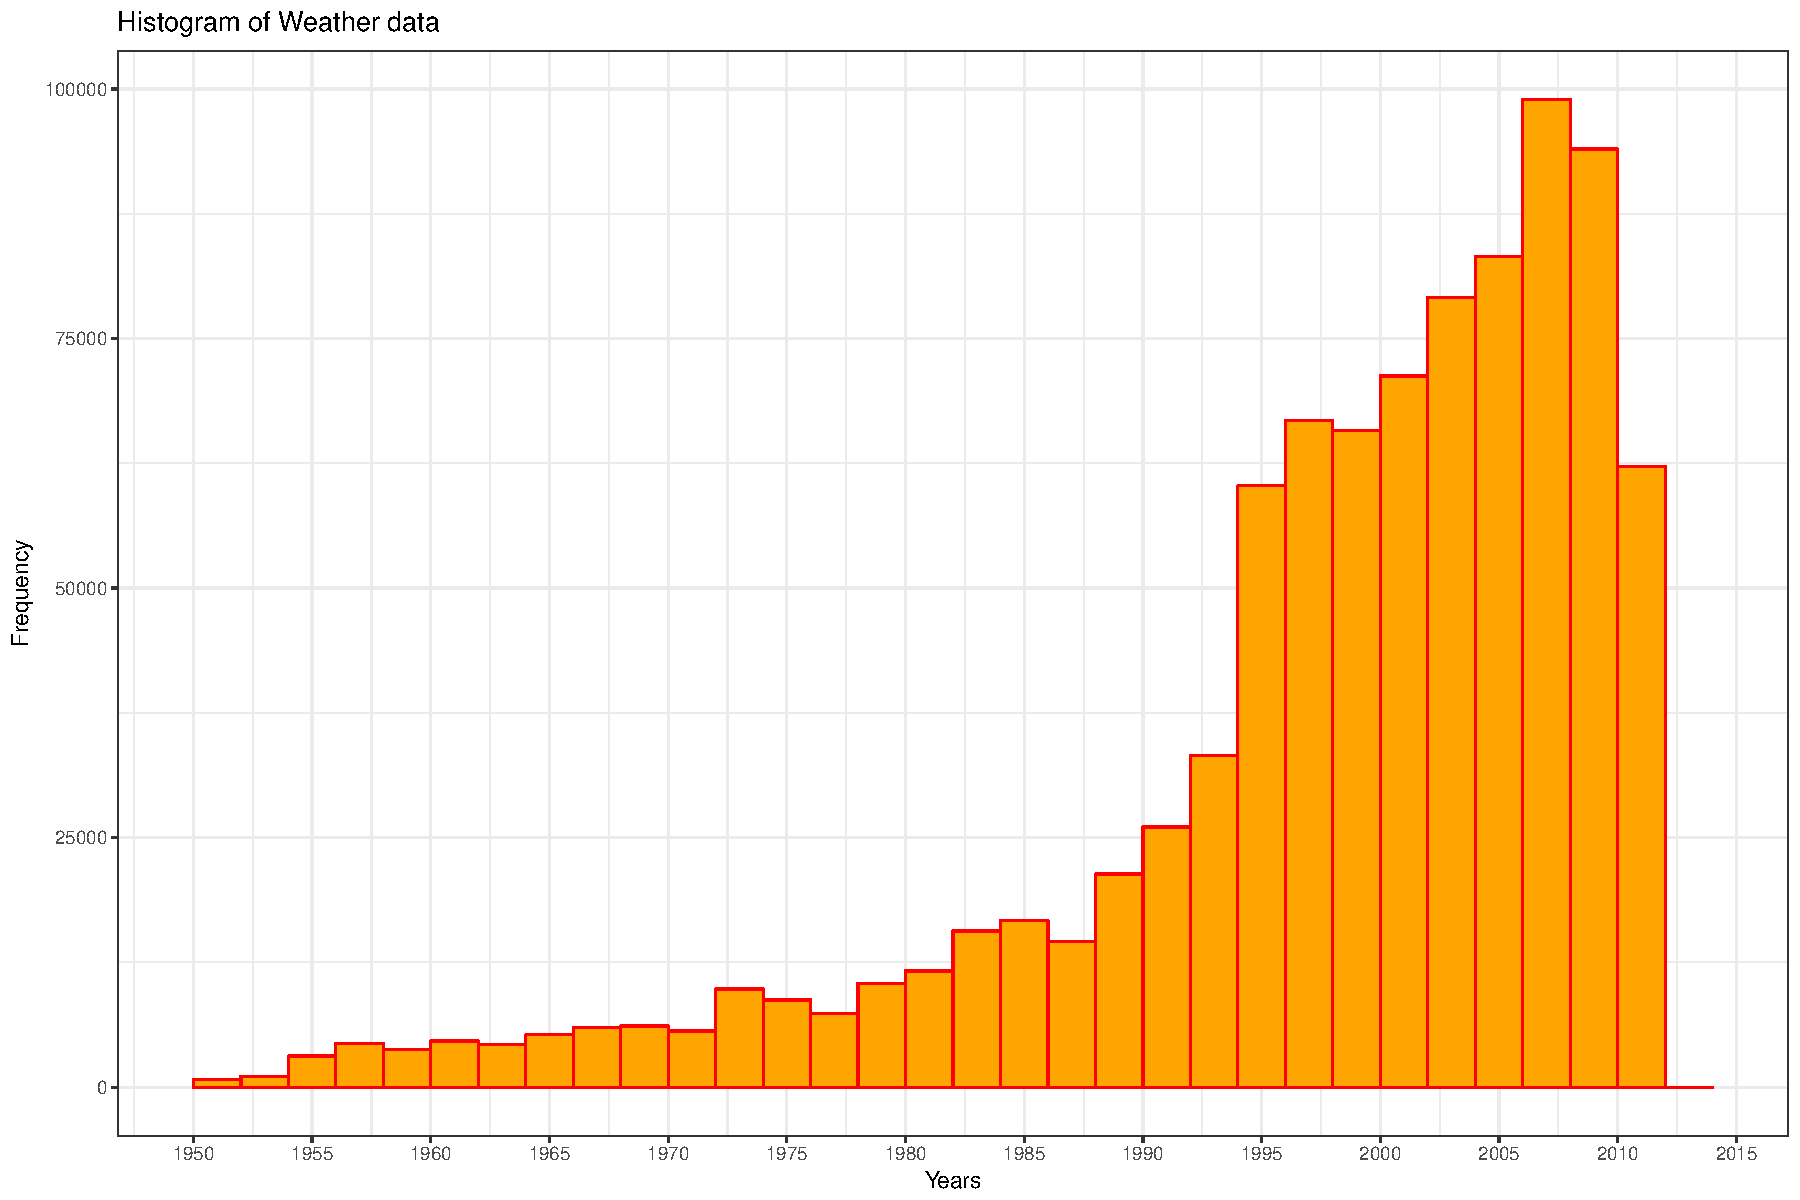
\includegraphics{NOAAStormDataAnalysis_files/figure-latex/unnamed-chunk-7-1.pdf}

Based on the histogram, we can say that 1995 can be a suitable year to
set consider as CUT-OFF year.

\begin{Shaded}
\begin{Highlighting}[]
\NormalTok{CutOffYear <-}\StringTok{ }\DecValTok{1995}
\NormalTok{essentialStormData <-}\StringTok{ }\NormalTok{essentialStormData[essentialStormData$Year >}\StringTok{ }\NormalTok{CutOffYear,]}
\NormalTok{LastYear <-}\StringTok{ }\KeywordTok{max}\NormalTok{(essentialStormData$Year)}
\end{Highlighting}
\end{Shaded}

\paragraph{4.2 Identify and categorizing different
events}\label{identify-and-categorizing-different-events}

The storm data records details for 985 unique source events. This number
can be reduced grouping similar events. We will have 9 levels defined
which will cover the majority of the events.

\textbf{NOTE:}\\
We have ignored the following 171 events\\
a) summaries\\
b) OTHER/Other\\
c) specified as NONE\\
d) Seiche\\
e) do not specify clearly the event

\begin{Shaded}
\begin{Highlighting}[]
\NormalTok{StormDamageDataGroup  <-}\StringTok{ }\NormalTok{essentialStormData}

\NormalTok{StormDamageDataGroup[}\KeywordTok{grepl}\NormalTok{(}\StringTok{"precipitation|rain|hail|drizzle|wet|}
\StringTok{                           precip|burst|depression|fog|wall cloud"}\NormalTok{, }
                         \NormalTok{StormDamageDataGroup$EventType, }\DataTypeTok{ignore.case =} \OtherTok{TRUE}\NormalTok{), }
                   \StringTok{"DamageEventGroup"}\NormalTok{] <-}\StringTok{ "Precipitation & Fog"}

\NormalTok{StormDamageDataGroup[}\KeywordTok{grepl}\NormalTok{(}\StringTok{"dust|saharan|wind|storm|wnd|hurricane|typhoon"}\NormalTok{, }
                         \NormalTok{StormDamageDataGroup$EventType, }\DataTypeTok{ignore.case =} \OtherTok{TRUE}\NormalTok{), }
                   \StringTok{"DamageEventGroup"}\NormalTok{] <-}\StringTok{ "Wind & Storm"}

\NormalTok{StormDamageDataGroup[}\KeywordTok{grepl}\NormalTok{(}\StringTok{"slide|erosion|slump"}\NormalTok{, }
                         \NormalTok{StormDamageDataGroup$EventType, }\DataTypeTok{ignore.case =} \OtherTok{TRUE}\NormalTok{), }
                   \StringTok{"DamageEventGroup"}\NormalTok{] <-}\StringTok{ "Landslide & Erosion"}

\NormalTok{StormDamageDataGroup[}\KeywordTok{grepl}\NormalTok{(}\StringTok{"warmth|warm|heat|dry|hot|drought|thermia|}
\StringTok{                           temperature record|record temperature|record high"}\NormalTok{, }
                         \NormalTok{StormDamageDataGroup$EventType, }\DataTypeTok{ignore.case =} \OtherTok{TRUE}\NormalTok{), }
                   \StringTok{"DamageEventGroup"}\NormalTok{] <-}\StringTok{ "Heat & Drought"}

\NormalTok{StormDamageDataGroup[}\KeywordTok{grepl}\NormalTok{(}\StringTok{"cold|cool|ice|icy|frost|freeze|snow|winter|wintry|}
\StringTok{                           wintery|blizzard|chill|freezing|avalanche|glaze|sleet"}\NormalTok{, }
                         \NormalTok{StormDamageDataGroup$EventType, }\DataTypeTok{ignore.case =} \OtherTok{TRUE}\NormalTok{), }
                   \StringTok{"DamageEventGroup"}\NormalTok{] <-}\StringTok{ "Snow & Ice"}

\NormalTok{StormDamageDataGroup[}\KeywordTok{grepl}\NormalTok{(}\StringTok{"flood|surf|blow-out|swells|fld|dam break"}\NormalTok{, }
                         \NormalTok{StormDamageDataGroup$EventType, }\DataTypeTok{ignore.case =} \OtherTok{TRUE}\NormalTok{), }
                   \StringTok{"DamageEventGroup"}\NormalTok{] <-}\StringTok{ "Flooding & Dam breaks"}

\NormalTok{StormDamageDataGroup[}\KeywordTok{grepl}\NormalTok{(}\StringTok{"seas|high water|tide|tsunami|wave|current|marine|drowning"}\NormalTok{, }
                         \NormalTok{StormDamageDataGroup$EventType, }\DataTypeTok{ignore.case =} \OtherTok{TRUE}\NormalTok{), }
                   \StringTok{"DamageEventGroup"}\NormalTok{] <-}\StringTok{ "Seas & Oceanic affects"}

\NormalTok{StormDamageDataGroup[}\KeywordTok{grepl}\NormalTok{(}\StringTok{"tstm|thunderstorm|lightning|tornado|spout|funnel|whirlwind"}\NormalTok{, }
                         \NormalTok{StormDamageDataGroup$EventType, }\DataTypeTok{ignore.case =} \OtherTok{TRUE}\NormalTok{), }
                   \StringTok{"DamageEventGroup"}\NormalTok{] <-}\StringTok{ "Tornado & Thunderstorm"}

\NormalTok{StormDamageDataGroup[}\KeywordTok{grepl}\NormalTok{(}\StringTok{"fire|smoke|volcanic"}\NormalTok{, }
                         \NormalTok{StormDamageDataGroup$EventType, }\DataTypeTok{ignore.case =} \OtherTok{TRUE}\NormalTok{), }
                   \StringTok{"DamageEventGroup"}\NormalTok{] <-}\StringTok{ "Fire & Volcanic activity"}

\CommentTok{# remove uncategorized records (DamageEventGroup == NA) & cast as factor}
\NormalTok{StormDamageDataGroup <-}\StringTok{ }
\StringTok{     }\NormalTok{StormDamageDataGroup[}\KeywordTok{complete.cases}\NormalTok{(StormDamageDataGroup[, }\StringTok{"DamageEventGroup"}\NormalTok{]), ]}

\NormalTok{StormDamageDataGroup$DamageEventGroup <-}\StringTok{ }\KeywordTok{as.factor}\NormalTok{(StormDamageDataGroup$DamageEventGroup)}
\NormalTok{groups <-}\StringTok{ }\KeywordTok{levels}\NormalTok{(StormDamageDataGroup$DamageEventGroup)}
\end{Highlighting}
\end{Shaded}

These events are grouped in theo following categories:\\
Fire \& Volcanic activity, Flooding \& Dam breaks, Heat \& Drought,
Landslide \& Erosion, Precipitation \& Fog, Seas \& Oceanic affects,
Snow \& Ice, Tornado \& Thunderstorm, Wind \& Storm

\paragraph{4.3 Consolidate data for
results}\label{consolidate-data-for-results}

\textbf{Here we are preparing the data for the Plots}\\
- \textbf{Step 1:} Aggregate the Property and Crop damage as Economic
damage

\begin{Shaded}
\begin{Highlighting}[]
\NormalTok{TotalEconomicDamage <-}\StringTok{ }\KeywordTok{aggregate}\NormalTok{(}\KeywordTok{cbind}\NormalTok{(PropertyDamageNew, CropDamageNew) ~}\StringTok{ }\NormalTok{DamageEventGroup, }
                                 \DataTypeTok{data=}\NormalTok{StormDamageDataGroup, }\DataTypeTok{FUN=}\NormalTok{sum, }\DataTypeTok{na.rm=}\OtherTok{TRUE}\NormalTok{)}

\NormalTok{TotalEconomicDamage <-}\StringTok{ }\NormalTok{TotalEconomicDamage[}\KeywordTok{order}\NormalTok{(TotalEconomicDamage$CropDamageNew, }
                                                 \DataTypeTok{decreasing=}\OtherTok{TRUE}\NormalTok{),]}

\KeywordTok{rownames}\NormalTok{(TotalEconomicDamage$DamageEventGroup) <-}\StringTok{ }\OtherTok{NULL}
\NormalTok{TotalEconomicDamage$DamageEventGroup <-}\StringTok{ }
\StringTok{     }\KeywordTok{factor}\NormalTok{(TotalEconomicDamage$DamageEventGroup,}
            \DataTypeTok{levels =} \KeywordTok{rev}\NormalTok{(TotalEconomicDamage$DamageEventGroup))}
\end{Highlighting}
\end{Shaded}

\begin{itemize}
\tightlist
\item
  \textbf{Step 2:} Aggregate the Fatalities and Injuries damage as Life
  damage
\end{itemize}

\begin{Shaded}
\begin{Highlighting}[]
\NormalTok{TotalLifeDamage <-}\StringTok{ }\KeywordTok{aggregate}\NormalTok{(}\KeywordTok{cbind}\NormalTok{(Fatalities,Injuries) ~}\StringTok{ }\NormalTok{DamageEventGroup, }
                             \DataTypeTok{data=}\NormalTok{StormDamageDataGroup, }
                             \DataTypeTok{FUN=}\NormalTok{sum, }\DataTypeTok{na.rm=}\OtherTok{TRUE}\NormalTok{)}

\NormalTok{TotalLifeDamage <-}\StringTok{ }\NormalTok{TotalLifeDamage[}\KeywordTok{order}\NormalTok{(TotalLifeDamage$Injuries, }
                                         \DataTypeTok{decreasing=}\OtherTok{TRUE}\NormalTok{),]}

\KeywordTok{rownames}\NormalTok{(TotalLifeDamage$DamageEventGroup) <-}\StringTok{ }\OtherTok{NULL}
\NormalTok{TotalLifeDamage$DamageEventGroup <-}\StringTok{ }
\StringTok{     }\KeywordTok{factor}\NormalTok{(TotalLifeDamage$DamageEventGroup, }
            \DataTypeTok{levels =} \KeywordTok{rev}\NormalTok{(TotalLifeDamage$DamageEventGroup))}
\end{Highlighting}
\end{Shaded}

\subsubsection{5. Summary - Life Damage}\label{summary---life-damage}

\paragraph{5.1 The results for Economic Damage - Property and
Crop}\label{the-results-for-economic-damage---property-and-crop}

\begin{verbatim}
##   DamageEventGroup         PropertyDamageNew CropDamageNew
## 3 Heat & Drought             1057077300      13860159500  
## 9 Wind & Storm             137990482290       6729948600  
## 2 Flooding & Dam breaks    159875724170       6349563200  
## 5 Precipitation & Fog       15203426360       3225242250  
## 7 Snow & Ice                 6467844450       2816170100  
## 8 Tornado & Thunderstorm    33285359370       1307316050  
## 1 Fire & Volcanic activity   7761049500        402255130  
## 6 Seas & Oceanic affects     4798122340         41022500  
## 4 Landslide & Erosion         327494100         20017000
\end{verbatim}

\paragraph{5.2 The results for Life Damage - Injuries and
Fatalities}\label{the-results-for-life-damage---injuries-and-fatalities}

\begin{verbatim}
##   DamageEventGroup         Fatalities Injuries
## 8 Tornado & Thunderstorm   2563       29975   
## 2 Flooding & Dam breaks    1483        8760   
## 3 Heat & Drought           2047        7644   
## 7 Snow & Ice               1150        3873   
## 9 Wind & Storm              569        3605   
## 5 Precipitation & Fog       170        1812   
## 1 Fire & Volcanic activity   87        1458   
## 6 Seas & Oceanic affects    618         763   
## 4 Landslide & Erosion        43          55
\end{verbatim}

\subsubsection{6. Plots}\label{plots}

\paragraph{6.1 Preparation}\label{preparation}

\begin{enumerate}
\def\labelenumi{\arabic{enumi})}
\tightlist
\item
  The plots for Life and Economic damages will be prepared using
  ggplot.\\
\item
  Each of the bar chart will have 3 plots

  \begin{enumerate}
  \def\labelenumii{\alph{enumii})}
  \tightlist
  \item
    1 plot will have only the Labels of weather events\\
  \item
    1 plot for each of the categories (Life: Fatalities Vs Injuries,
    Economic: Property Vs Crop)\\
  \end{enumerate}
\item
  The bar chart will have a layout: \textbf{Data plot 1 - Label Plot -
  Data Plot 2}\\
\item
  Two new functions are written to help prepare the layout and include
  the plot in the layout

  \begin{enumerate}
  \def\labelenumii{\alph{enumii})}
  \tightlist
  \item
    \textbf{multiplot} function will create the new grid page and set up
    the view\\
  \item
    \textbf{plotLayout} function will set tup the plots as per the given
    coordinates
  \end{enumerate}
\end{enumerate}

\begin{Shaded}
\begin{Highlighting}[]
\CommentTok{# The layout for plot on Life damages}
\NormalTok{Layout1 =}\StringTok{ }\KeywordTok{grid.layout}\NormalTok{(}\DecValTok{2}\NormalTok{, }\DecValTok{3}\NormalTok{, }\DataTypeTok{heights =} \KeywordTok{unit}\NormalTok{(}\KeywordTok{c}\NormalTok{(}\FloatTok{0.3}\NormalTok{,}\DecValTok{7}\NormalTok{), }\StringTok{"inches"}\NormalTok{),}
                      \DataTypeTok{widths =} \KeywordTok{unit}\NormalTok{(}\KeywordTok{c}\NormalTok{(}\DecValTok{4}\NormalTok{,}\FloatTok{2.5}\NormalTok{,}\DecValTok{4}\NormalTok{), }\StringTok{"inches"}\NormalTok{))}

\CommentTok{# The layout for plot on Economic damages}
\NormalTok{Layout2 =}\StringTok{ }\KeywordTok{grid.layout}\NormalTok{(}\DecValTok{2}\NormalTok{, }\DecValTok{3}\NormalTok{, }\DataTypeTok{heights =} \KeywordTok{unit}\NormalTok{(}\KeywordTok{c}\NormalTok{(}\FloatTok{0.3}\NormalTok{,}\DecValTok{7}\NormalTok{), }\StringTok{"inches"}\NormalTok{), }
                      \DataTypeTok{widths =} \KeywordTok{unit}\NormalTok{(}\KeywordTok{c}\NormalTok{(}\DecValTok{4}\NormalTok{,}\DecValTok{2}\NormalTok{,}\DecValTok{4}\NormalTok{), }\StringTok{"inches"}\NormalTok{))}

\CommentTok{# plotLayout function will set tup the plots as per the given coordinates}
\NormalTok{plotLayout <-}\StringTok{ }\NormalTok{function(x, y) }\KeywordTok{viewport}\NormalTok{(}\DataTypeTok{layout.pos.row =} \NormalTok{x,}
                                   \DataTypeTok{layout.pos.col =} \NormalTok{y)}

\CommentTok{# multiplot function will create the new grid page and set up the view  }
\NormalTok{multiplot <-}\StringTok{ }\NormalTok{function(Layout, a, b, c, d) \{}
     \KeywordTok{grid.newpage}\NormalTok{()}
     \KeywordTok{pushViewport}\NormalTok{(}\KeywordTok{viewport}\NormalTok{(}\DataTypeTok{layout =} \NormalTok{Layout))}
     \KeywordTok{grid.text}\NormalTok{(a, }\DataTypeTok{vp =} \KeywordTok{viewport}\NormalTok{(}\DataTypeTok{layout.pos.row =} \DecValTok{1}\NormalTok{, }\DataTypeTok{layout.pos.col =} \DecValTok{1}\NormalTok{:}\DecValTok{3}\NormalTok{))}
     \KeywordTok{print}\NormalTok{(b, }\DataTypeTok{vp =} \KeywordTok{plotLayout}\NormalTok{(}\DecValTok{2}\NormalTok{, }\DecValTok{1}\NormalTok{))}
     \KeywordTok{print}\NormalTok{(c, }\DataTypeTok{vp =} \KeywordTok{plotLayout}\NormalTok{(}\DecValTok{2}\NormalTok{, }\DecValTok{2}\NormalTok{))}
     \KeywordTok{print}\NormalTok{(d, }\DataTypeTok{vp =} \KeywordTok{plotLayout}\NormalTok{(}\DecValTok{2}\NormalTok{, }\DecValTok{3}\NormalTok{))}
\NormalTok{\}}
\end{Highlighting}
\end{Shaded}

\paragraph{6.2 Life Damages - Injuries Vs.
Fatalities}\label{life-damages---injuries-vs.-fatalities}

Please see below the code and plot for Damages to human life due to
severe weather events, resulting in Death and injuries.

\begin{Shaded}
\begin{Highlighting}[]
\NormalTok{plotTitle1 =}\StringTok{ }\KeywordTok{paste}\NormalTok{(}\KeywordTok{c}\NormalTok{(}\StringTok{"Injuries & Fatalities to humans due to weather events from:"}\NormalTok{,}
                     \NormalTok{CutOffYear,}\StringTok{" to:"}\NormalTok{,LastYear), }
                   \DataTypeTok{collapse =} \StringTok{" "}\NormalTok{)}
\NormalTok{g.LifeLabels <-}\StringTok{ }\KeywordTok{ggplot}\NormalTok{(}\DataTypeTok{data=}\NormalTok{TotalLifeDamage, }
                       \KeywordTok{aes}\NormalTok{(}\DataTypeTok{x=}\DecValTok{1}\NormalTok{,}\DataTypeTok{y=}\NormalTok{DamageEventGroup)) +}
\StringTok{     }\KeywordTok{geom_text}\NormalTok{(}\KeywordTok{aes}\NormalTok{(}\DataTypeTok{label=}\NormalTok{DamageEventGroup), }\DataTypeTok{size=}\DecValTok{4}\NormalTok{) +}
\StringTok{     }\KeywordTok{ggtitle}\NormalTok{(}\StringTok{""}\NormalTok{) +}
\StringTok{     }\KeywordTok{ylab}\NormalTok{(}\OtherTok{NULL}\NormalTok{) +}
\StringTok{     }\KeywordTok{scale_x_continuous}\NormalTok{(}\DataTypeTok{expand=}\KeywordTok{c}\NormalTok{(}\DecValTok{0}\NormalTok{,}\DecValTok{0}\NormalTok{),}\DataTypeTok{limits=}\KeywordTok{c}\NormalTok{(}\DecValTok{1}\NormalTok{,}\DecValTok{1}\NormalTok{)) +}
\StringTok{     }\KeywordTok{theme}\NormalTok{(}\DataTypeTok{axis.title=}\KeywordTok{element_blank}\NormalTok{(),}
           \DataTypeTok{panel.grid=}\KeywordTok{element_blank}\NormalTok{(),}
           \DataTypeTok{axis.text.y=}\KeywordTok{element_blank}\NormalTok{(),}
           \DataTypeTok{axis.ticks.y=}\KeywordTok{element_blank}\NormalTok{(),}
           \DataTypeTok{panel.background=}\KeywordTok{element_blank}\NormalTok{(),}
           \DataTypeTok{axis.text.x=}\KeywordTok{element_text}\NormalTok{(}\DataTypeTok{color=}\OtherTok{NA}\NormalTok{),}
           \DataTypeTok{axis.ticks.x=}\KeywordTok{element_line}\NormalTok{(}\DataTypeTok{color=}\OtherTok{NA}\NormalTok{))}

\CommentTok{# Plot chart with injuries}
\NormalTok{yLim1 <-}\StringTok{ }\KeywordTok{max}\NormalTok{(TotalLifeDamage$Injuries}\DecValTok{+100}\NormalTok{)}
\NormalTok{g.Injuries <-}\StringTok{ }\KeywordTok{ggplot}\NormalTok{(}\DataTypeTok{data=}\NormalTok{TotalLifeDamage, }
                     \KeywordTok{aes}\NormalTok{(}\DataTypeTok{x=}\NormalTok{DamageEventGroup, }
                         \DataTypeTok{y=}\NormalTok{Injuries),}
                         \DataTypeTok{fill =} \KeywordTok{factor}\NormalTok{(Injuries)) +}
\StringTok{     }\KeywordTok{geom_bar}\NormalTok{(}\DataTypeTok{stat =} \StringTok{"identity"}\NormalTok{, }\KeywordTok{aes}\NormalTok{(}\DataTypeTok{fill =} \KeywordTok{factor}\NormalTok{(DamageEventGroup))) +}\StringTok{ }
\StringTok{     }\KeywordTok{geom_text}\NormalTok{(}\KeywordTok{aes}\NormalTok{(}\DataTypeTok{label=}\NormalTok{Injuries), }\DataTypeTok{size=}\DecValTok{3}\NormalTok{, }\DataTypeTok{vjust=}\FloatTok{0.5}\NormalTok{, }\DataTypeTok{hjust=}\FloatTok{0.0}\NormalTok{) +}
\StringTok{     }\KeywordTok{ggtitle}\NormalTok{(}\StringTok{"Injuries"}\NormalTok{) +}
\StringTok{     }\KeywordTok{scale_y_continuous}\NormalTok{(}\DataTypeTok{limits =} \KeywordTok{c}\NormalTok{(}\DecValTok{0}\NormalTok{,yLim1), }\DataTypeTok{breaks =} \KeywordTok{seq}\NormalTok{(}\DecValTok{0}\NormalTok{,yLim1,}\DecValTok{5000}\NormalTok{)) +}
\StringTok{     }\KeywordTok{coord_flip}\NormalTok{() +}
\StringTok{     }\KeywordTok{theme}\NormalTok{(}\DataTypeTok{axis.title.x =} \KeywordTok{element_blank}\NormalTok{(), }
           \DataTypeTok{axis.title.y =} \KeywordTok{element_blank}\NormalTok{(), }
           \DataTypeTok{axis.text.y =} \KeywordTok{element_blank}\NormalTok{(), }
           \DataTypeTok{axis.ticks.y =} \KeywordTok{element_blank}\NormalTok{(), }
           \DataTypeTok{legend.position =} \StringTok{"none"}\NormalTok{)}

\CommentTok{# Plot chart with fatalities}
\NormalTok{yLim2 <-}\StringTok{ }\KeywordTok{max}\NormalTok{(TotalLifeDamage$Fatalities}\DecValTok{+100}\NormalTok{)}
\NormalTok{g.Fatalities <-}\StringTok{ }\KeywordTok{ggplot}\NormalTok{(}\DataTypeTok{data=}\NormalTok{TotalLifeDamage, }
                       \KeywordTok{aes}\NormalTok{(}\DataTypeTok{x=}\NormalTok{DamageEventGroup, }
                           \DataTypeTok{y=}\NormalTok{Fatalities, }
                           \DataTypeTok{fill =} \KeywordTok{factor}\NormalTok{(DamageEventGroup))) +}
\StringTok{     }\KeywordTok{geom_bar}\NormalTok{(}\DataTypeTok{stat =} \StringTok{"identity"}\NormalTok{) +}\StringTok{ }
\StringTok{     }\KeywordTok{geom_text}\NormalTok{(}\KeywordTok{aes}\NormalTok{(}\DataTypeTok{label=}\NormalTok{Fatalities), }\DataTypeTok{size=}\DecValTok{3}\NormalTok{, }\DataTypeTok{vjust=}\FloatTok{0.5}\NormalTok{, }\DataTypeTok{hjust=}\FloatTok{0.0}\NormalTok{) +}
\StringTok{     }\KeywordTok{ggtitle}\NormalTok{(}\StringTok{"Fatalities"}\NormalTok{) +}
\StringTok{     }\KeywordTok{coord_flip}\NormalTok{() +}
\StringTok{     }\KeywordTok{scale_y_continuous}\NormalTok{(}\DataTypeTok{limits =} \KeywordTok{c}\NormalTok{(}\DecValTok{0}\NormalTok{,yLim2), }\DataTypeTok{breaks =} \KeywordTok{seq}\NormalTok{(}\DecValTok{0}\NormalTok{, yLim2, }\DecValTok{500}\NormalTok{)) +}
\StringTok{     }\KeywordTok{theme}\NormalTok{(}\DataTypeTok{axis.title.x =} \KeywordTok{element_blank}\NormalTok{(), }
           \DataTypeTok{axis.title.y =} \KeywordTok{element_blank}\NormalTok{(), }
           \DataTypeTok{axis.text.y =} \KeywordTok{element_blank}\NormalTok{(), }
           \DataTypeTok{axis.ticks.y =} \KeywordTok{element_blank}\NormalTok{(), }
           \DataTypeTok{legend.position =} \StringTok{"none"}\NormalTok{)}

\CommentTok{# We will combine both the plots in to one.}
\KeywordTok{multiplot}\NormalTok{(Layout1, plotTitle1,  g.Injuries, g.LifeLabels, g.Fatalities)}
\end{Highlighting}
\end{Shaded}

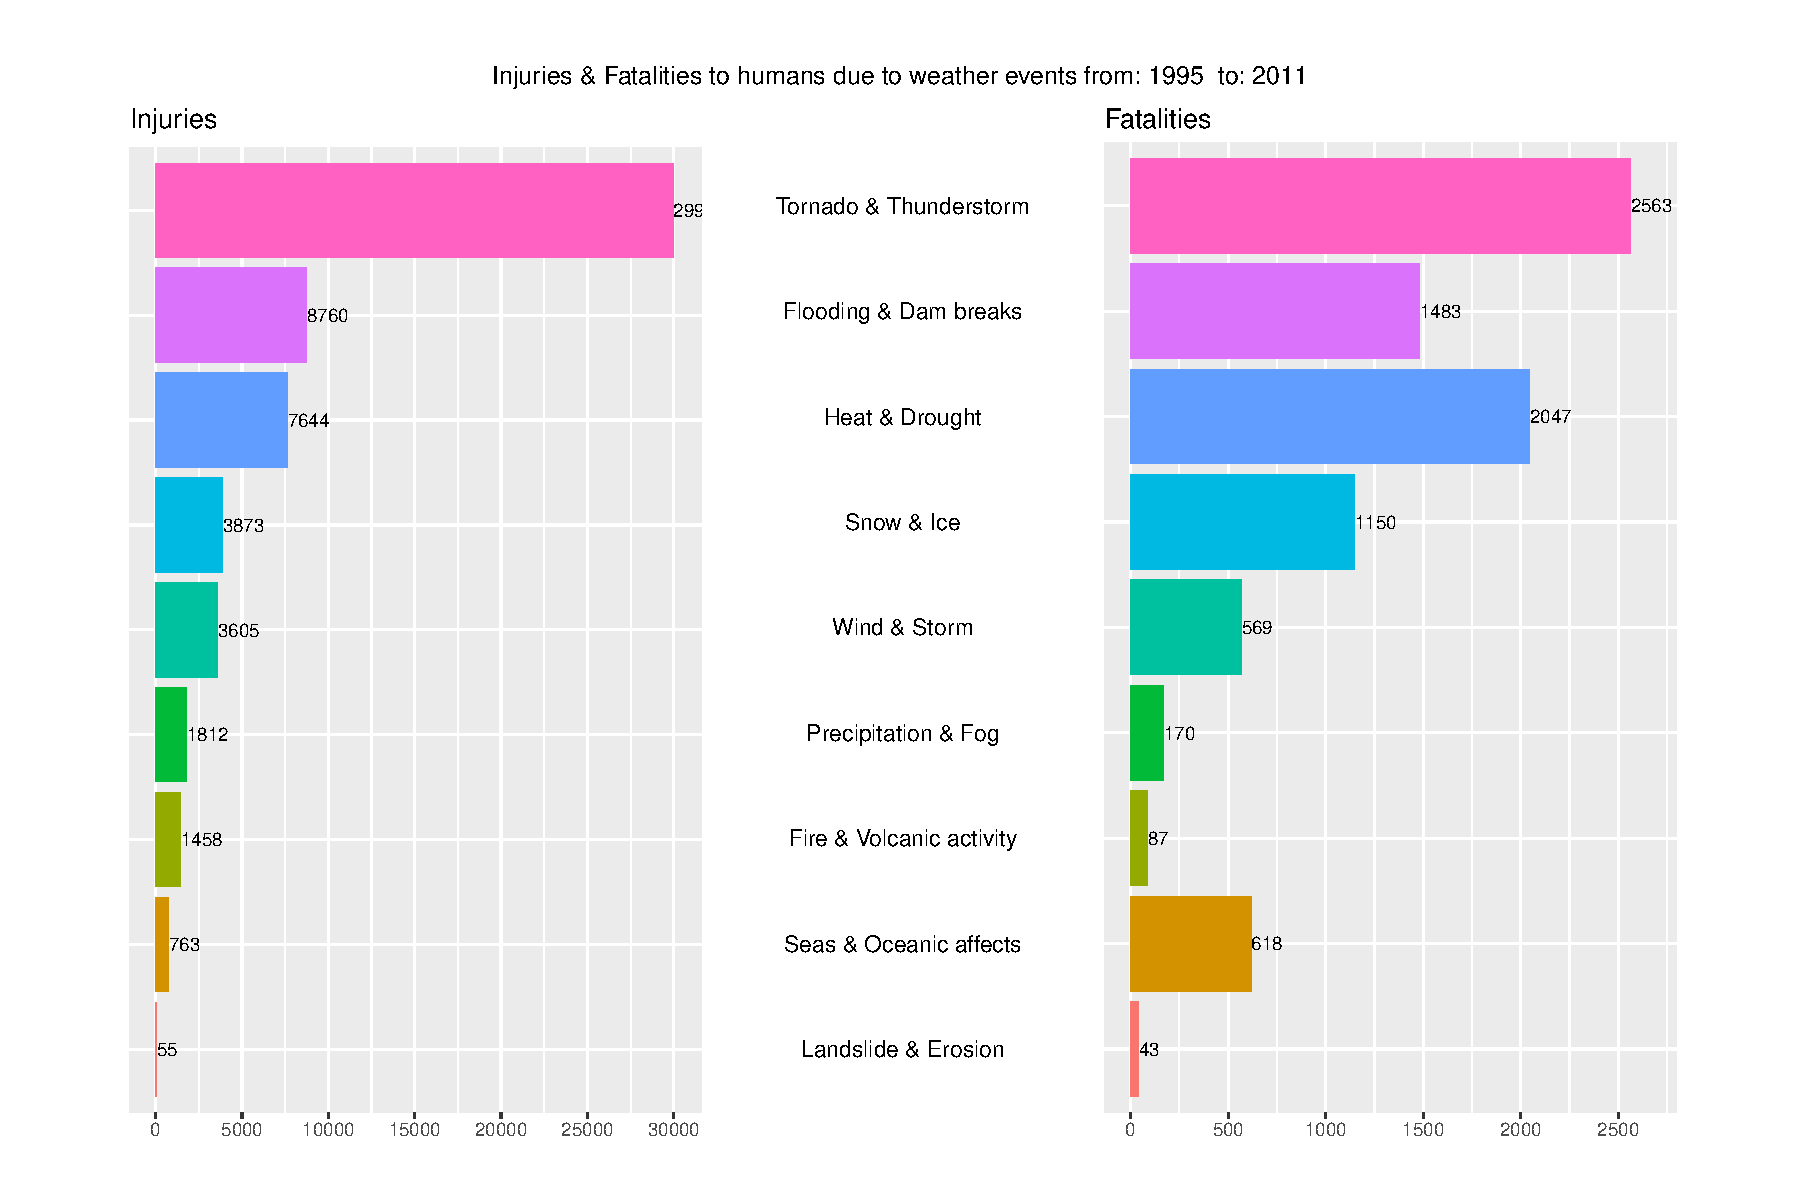
\includegraphics{NOAAStormDataAnalysis_files/figure-latex/unnamed-chunk-15-1.pdf}

\paragraph{6.3 Economic Damages - Property \&
Crop}\label{economic-damages---property-crop}

Please see below the code and plot for Economic Damages to Property Vs
Crop due to severe weather events

\begin{Shaded}
\begin{Highlighting}[]
\NormalTok{plotTitle2 =}\StringTok{ }\KeywordTok{paste}\NormalTok{(}\KeywordTok{c}\NormalTok{(}\StringTok{"Damage to Crops and Property due to weather events from:"}\NormalTok{,}
                     \NormalTok{CutOffYear,}\StringTok{" to:"}\NormalTok{,LastYear), }
                   \DataTypeTok{collapse =} \StringTok{" "}\NormalTok{)}

\CommentTok{# Plot chart with Damage group labels  }
\NormalTok{g.EconLabels <-}\StringTok{ }\KeywordTok{ggplot}\NormalTok{(}\DataTypeTok{data=}\NormalTok{TotalEconomicDamage, }
                       \KeywordTok{aes}\NormalTok{(}\DataTypeTok{x=}\DecValTok{1}\NormalTok{,}\DataTypeTok{y=}\NormalTok{DamageEventGroup)) +}
\StringTok{     }\KeywordTok{geom_text}\NormalTok{(}\KeywordTok{aes}\NormalTok{(}\DataTypeTok{label=}\NormalTok{DamageEventGroup), }\DataTypeTok{size=}\DecValTok{4}\NormalTok{) +}
\StringTok{     }\KeywordTok{ggtitle}\NormalTok{(}\StringTok{""}\NormalTok{) +}
\StringTok{     }\KeywordTok{ylab}\NormalTok{(}\OtherTok{NULL}\NormalTok{) +}
\StringTok{     }\KeywordTok{scale_x_continuous}\NormalTok{(}\DataTypeTok{expand=}\KeywordTok{c}\NormalTok{(}\DecValTok{0}\NormalTok{,}\DecValTok{0}\NormalTok{),}\DataTypeTok{limits=}\KeywordTok{c}\NormalTok{(}\DecValTok{1}\NormalTok{,}\DecValTok{1}\NormalTok{)) +}
\StringTok{     }\KeywordTok{theme}\NormalTok{(}\DataTypeTok{axis.title=}\KeywordTok{element_blank}\NormalTok{(),}
           \DataTypeTok{panel.grid=}\KeywordTok{element_blank}\NormalTok{(),}
           \DataTypeTok{axis.text.y=}\KeywordTok{element_blank}\NormalTok{(),}
           \DataTypeTok{axis.ticks.y=}\KeywordTok{element_blank}\NormalTok{(),}
           \DataTypeTok{panel.background=}\KeywordTok{element_blank}\NormalTok{(),}
           \DataTypeTok{axis.text.x=}\KeywordTok{element_text}\NormalTok{(}\DataTypeTok{color=}\OtherTok{NA}\NormalTok{),}
           \DataTypeTok{axis.ticks.x=}\KeywordTok{element_line}\NormalTok{(}\DataTypeTok{color=}\OtherTok{NA}\NormalTok{),}
           \DataTypeTok{plot.margin =} \KeywordTok{unit}\NormalTok{(}\KeywordTok{c}\NormalTok{(}\DecValTok{0}\NormalTok{,}\DecValTok{0}\NormalTok{,}\DecValTok{0}\NormalTok{,}\DecValTok{0}\NormalTok{), }\StringTok{"mm"}\NormalTok{))}

\CommentTok{# Plot chart with Property damages}
\NormalTok{yLim3 <-}\StringTok{ }\KeywordTok{max}\NormalTok{((TotalEconomicDamage$PropertyDamageNew/}\DecValTok{1000000}\NormalTok{)+}\DecValTok{500}\NormalTok{)}
\NormalTok{g.Property <-}\StringTok{ }\KeywordTok{ggplot}\NormalTok{(}\DataTypeTok{data=}\NormalTok{TotalEconomicDamage, }
                     \KeywordTok{aes}\NormalTok{(}\DataTypeTok{x=}\NormalTok{DamageEventGroup, }
                         \DataTypeTok{y=}\NormalTok{PropertyDamageNew/}\DecValTok{1000000}\NormalTok{, }
                         \DataTypeTok{label=}\KeywordTok{sprintf}\NormalTok{(}\StringTok{"%0.2f"}\NormalTok{, }
                                       \KeywordTok{round}\NormalTok{(PropertyDamageNew/}\DecValTok{1000000}\NormalTok{, }
                                             \DataTypeTok{digits =} \DecValTok{2}\NormalTok{))),}
                     \DataTypeTok{fill =} \KeywordTok{factor}\NormalTok{(}\KeywordTok{round}\NormalTok{(PropertyDamageNew/}\DecValTok{1000000}\NormalTok{, }
                                         \DataTypeTok{digits =} \DecValTok{2}\NormalTok{))) +}
\StringTok{     }\KeywordTok{geom_bar}\NormalTok{(}\DataTypeTok{stat =} \StringTok{"identity"}\NormalTok{, }\KeywordTok{aes}\NormalTok{(}\DataTypeTok{fill =} \KeywordTok{factor}\NormalTok{(DamageEventGroup))) +}\StringTok{ }
\StringTok{     }\KeywordTok{geom_text}\NormalTok{(}\DataTypeTok{size=}\DecValTok{3}\NormalTok{, }\KeywordTok{aes}\NormalTok{(}\DataTypeTok{label=}\KeywordTok{round}\NormalTok{(PropertyDamageNew/}\DecValTok{1000000}\NormalTok{, }
                                       \DataTypeTok{digits =} \DecValTok{2}\NormalTok{)),}
               \DataTypeTok{vjust=}\FloatTok{0.0}\NormalTok{, }\DataTypeTok{hjust=}\FloatTok{0.5}\NormalTok{) +}
\StringTok{     }\KeywordTok{ggtitle}\NormalTok{(}\StringTok{"Property Damage (in USD million)"}\NormalTok{) +}
\StringTok{     }\KeywordTok{scale_y_continuous}\NormalTok{(}\DataTypeTok{limits =} \KeywordTok{c}\NormalTok{(}\DecValTok{0}\NormalTok{,yLim3), }\DataTypeTok{breaks =} \KeywordTok{seq}\NormalTok{(}\DecValTok{0}\NormalTok{,yLim3,}\DecValTok{25000}\NormalTok{)) +}
\StringTok{     }\KeywordTok{coord_flip}\NormalTok{() +}
\StringTok{     }\KeywordTok{theme}\NormalTok{(}\DataTypeTok{axis.title.x =} \KeywordTok{element_blank}\NormalTok{(), }
           \DataTypeTok{axis.title.y =} \KeywordTok{element_blank}\NormalTok{(), }
           \DataTypeTok{axis.text.y =} \KeywordTok{element_blank}\NormalTok{(), }
           \DataTypeTok{axis.ticks.y =} \KeywordTok{element_blank}\NormalTok{(), }
           \DataTypeTok{legend.position =} \StringTok{"none"}\NormalTok{)}

\CommentTok{# Plot chart with Crop damages  }
\NormalTok{yLim4 <-}\StringTok{ }\KeywordTok{max}\NormalTok{((TotalEconomicDamage$CropDamageNew/}\DecValTok{1000000}\NormalTok{)+}\DecValTok{100}\NormalTok{)}
\NormalTok{g.Crop <-}\StringTok{ }\KeywordTok{ggplot}\NormalTok{(}\DataTypeTok{data=}\NormalTok{TotalEconomicDamage, }
                 \KeywordTok{aes}\NormalTok{(}\DataTypeTok{x=}\NormalTok{DamageEventGroup, }
                     \DataTypeTok{y=}\NormalTok{CropDamageNew/}\DecValTok{1000000}\NormalTok{,}
                     \DataTypeTok{label=}\KeywordTok{sprintf}\NormalTok{(}\StringTok{"%0.2f"}\NormalTok{, }
                                   \KeywordTok{round}\NormalTok{(CropDamageNew/}\DecValTok{1000000}\NormalTok{, }
                                         \DataTypeTok{digits =} \DecValTok{2}\NormalTok{))),}
                 \DataTypeTok{fill =} \KeywordTok{factor}\NormalTok{(}\KeywordTok{round}\NormalTok{(CropDamageNew/}\DecValTok{1000000}\NormalTok{, }
                                     \DataTypeTok{digits =} \DecValTok{2}\NormalTok{))) +}
\StringTok{     }\KeywordTok{geom_bar}\NormalTok{(}\DataTypeTok{stat =} \StringTok{"identity"}\NormalTok{, }\KeywordTok{aes}\NormalTok{(}\DataTypeTok{fill =} \KeywordTok{factor}\NormalTok{(DamageEventGroup))) +}\StringTok{ }
\StringTok{     }\KeywordTok{geom_text}\NormalTok{(}\DataTypeTok{size=}\DecValTok{3}\NormalTok{, }\KeywordTok{aes}\NormalTok{(}\DataTypeTok{label=}\KeywordTok{round}\NormalTok{(CropDamageNew/}\DecValTok{1000000}\NormalTok{, }
                                       \DataTypeTok{digits =} \DecValTok{2}\NormalTok{), }
                           \DataTypeTok{vjust=}\FloatTok{0.0}\NormalTok{, }\DataTypeTok{hjust=}\FloatTok{0.0}\NormalTok{)) +}
\StringTok{     }\KeywordTok{ggtitle}\NormalTok{(}\StringTok{"Crop Damage (in USD million)"}\NormalTok{) +}
\StringTok{     }\KeywordTok{scale_y_continuous}\NormalTok{(}\DataTypeTok{limits =} \KeywordTok{c}\NormalTok{(}\DecValTok{0}\NormalTok{,yLim4), }\DataTypeTok{breaks =} \KeywordTok{seq}\NormalTok{(}\DecValTok{0}\NormalTok{,yLim4,}\DecValTok{2000}\NormalTok{)) +}
\StringTok{     }\KeywordTok{coord_flip}\NormalTok{() +}
\StringTok{     }\KeywordTok{theme}\NormalTok{(}\DataTypeTok{axis.title.x =} \KeywordTok{element_blank}\NormalTok{(), }
           \DataTypeTok{axis.title.y =} \KeywordTok{element_blank}\NormalTok{(), }
           \DataTypeTok{axis.text.y =} \KeywordTok{element_blank}\NormalTok{(), }
           \DataTypeTok{axis.ticks.y =} \KeywordTok{element_blank}\NormalTok{(), }
           \DataTypeTok{legend.position =} \StringTok{"none"}\NormalTok{)}

\KeywordTok{multiplot}\NormalTok{(Layout2, plotTitle2, g.Crop, g.EconLabels,g.Property)}
\end{Highlighting}
\end{Shaded}

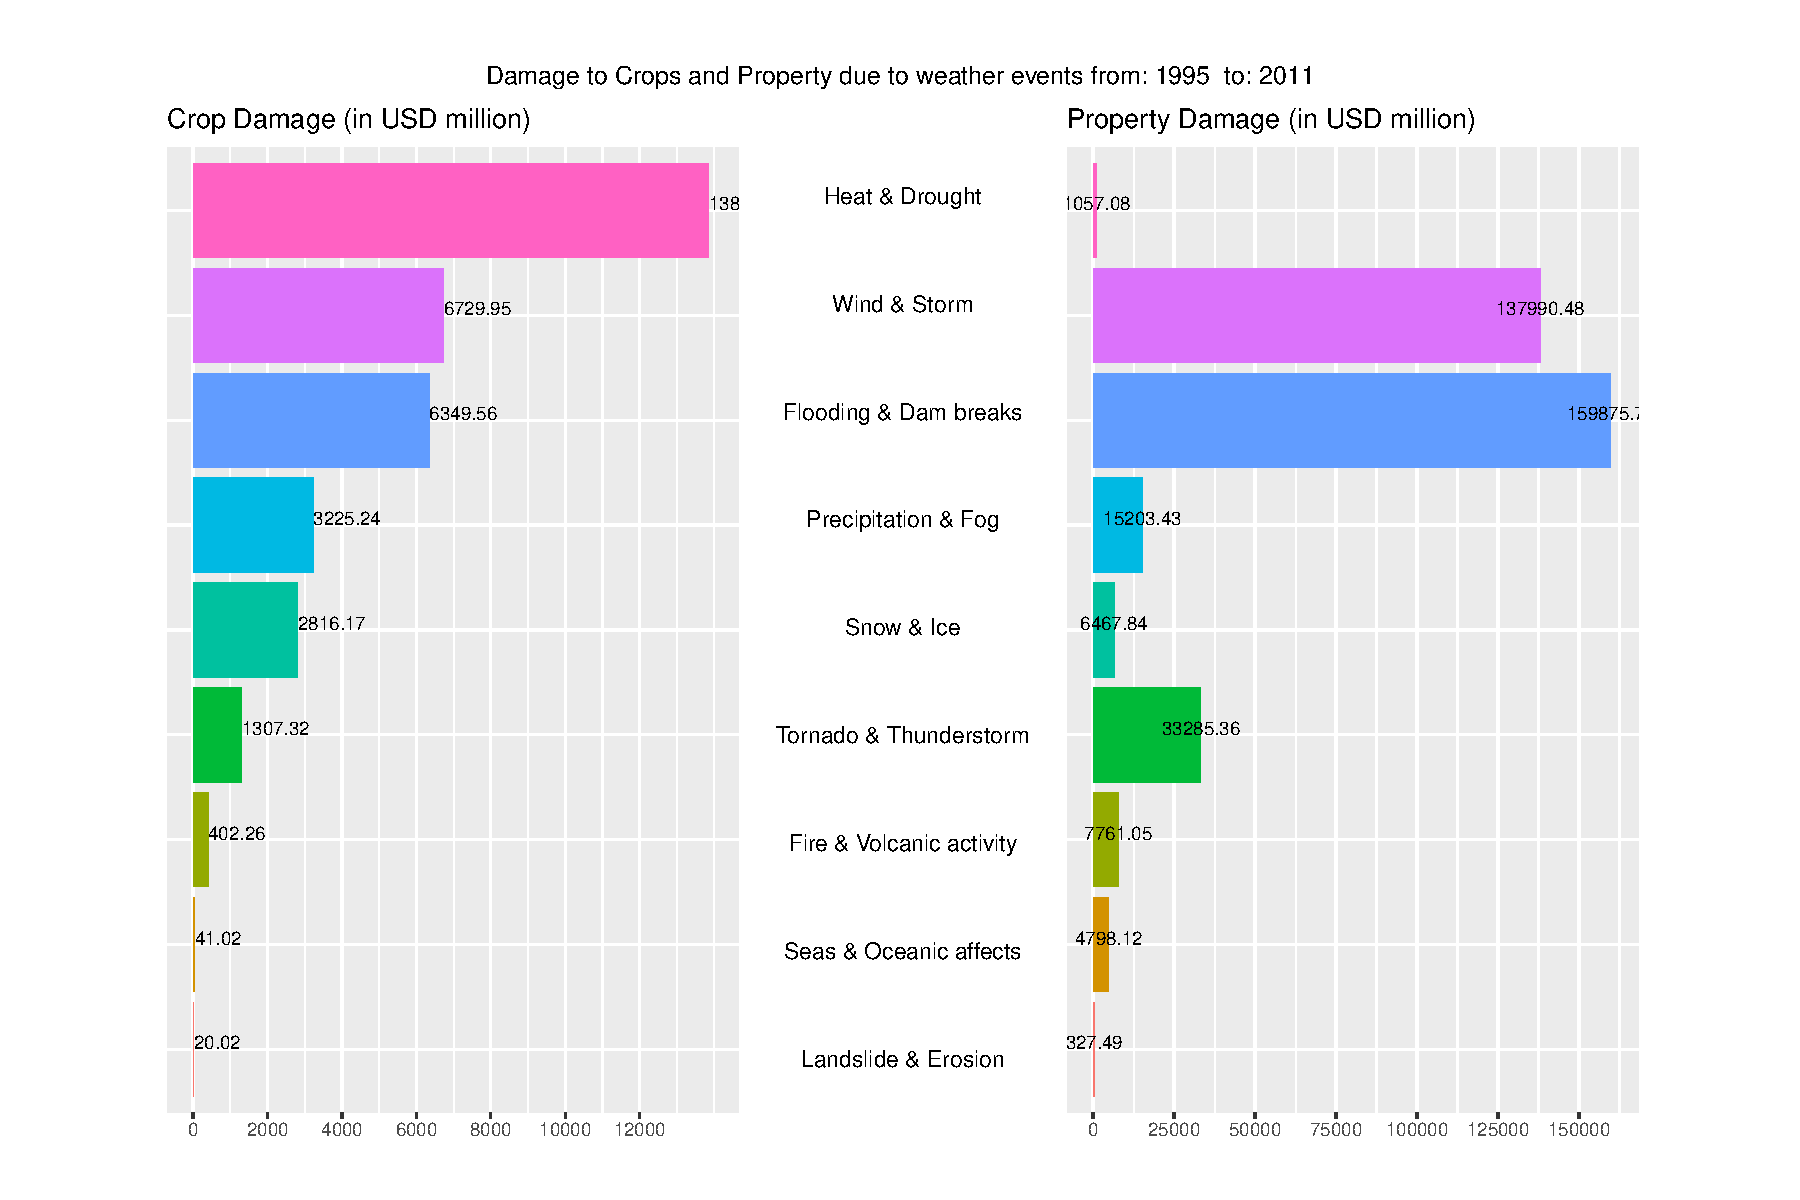
\includegraphics{NOAAStormDataAnalysis_files/figure-latex/unnamed-chunk-16-1.pdf}

\subsection{SUMMARY}\label{summary}

This is the summary of damages caused due to severe weather events
occured during the period \textbf{1995 to 2011}.

\subsubsection{A) Human Life Damages - Injuries \&
Fatalities}\label{a-human-life-damages---injuries-fatalities}

\begin{itemize}
\tightlist
\item
  The \textbf{Tornado, Thuderstorm \& Lightning} group has caused
  highest damages for human life in both the Fatalities and Injuries.
\end{itemize}

\subsubsection{B) Economic Damages - Property \&
Crop}\label{b-economic-damages---property-crop}

\begin{enumerate}
\def\labelenumi{\arabic{enumi})}
\tightlist
\item
  The \textbf{Heat \& Drought} group has caused highest damages for
  Crops with USD 13.86 billion\\
\item
  The \textbf{Flooding \& Dam breakages} group has caused highest
  damages for Property with USD 13.86 billion
\end{enumerate}

\subsubsection{C) Data used for this
analysis}\label{c-data-used-for-this-analysis}

\begin{itemize}
\tightlist
\item
  The data used for this analysis is stored and to reproduce the plot
  and results later.
\end{itemize}

\begin{Shaded}
\begin{Highlighting}[]
\KeywordTok{save}\NormalTok{(essentialStormData,}
     \NormalTok{StormDamageDataGroup,}
     \NormalTok{TotalEconomicDamage,}
     \NormalTok{TotalLifeDamage,}
     \NormalTok{CutOffYear,}
     \NormalTok{LastYear,}
     \DataTypeTok{file =} \StringTok{"./data/StormAnalysisData.RData"}\NormalTok{)}
\end{Highlighting}
\end{Shaded}

-----------------END OF ANALYSIS REPORT-------------------


\end{document}
